\chapter{Malaria and Malaria Models}

\section{Malaria}

Malaria kills around 600,000 people each year, with over 75\% of deaths
occurring in children under 5 years old
\parencite{world_health_organization_world_2022}.

\subsection*{Plasmodium Life Cycle}

\begin{figure}[htbp]
    \centering
    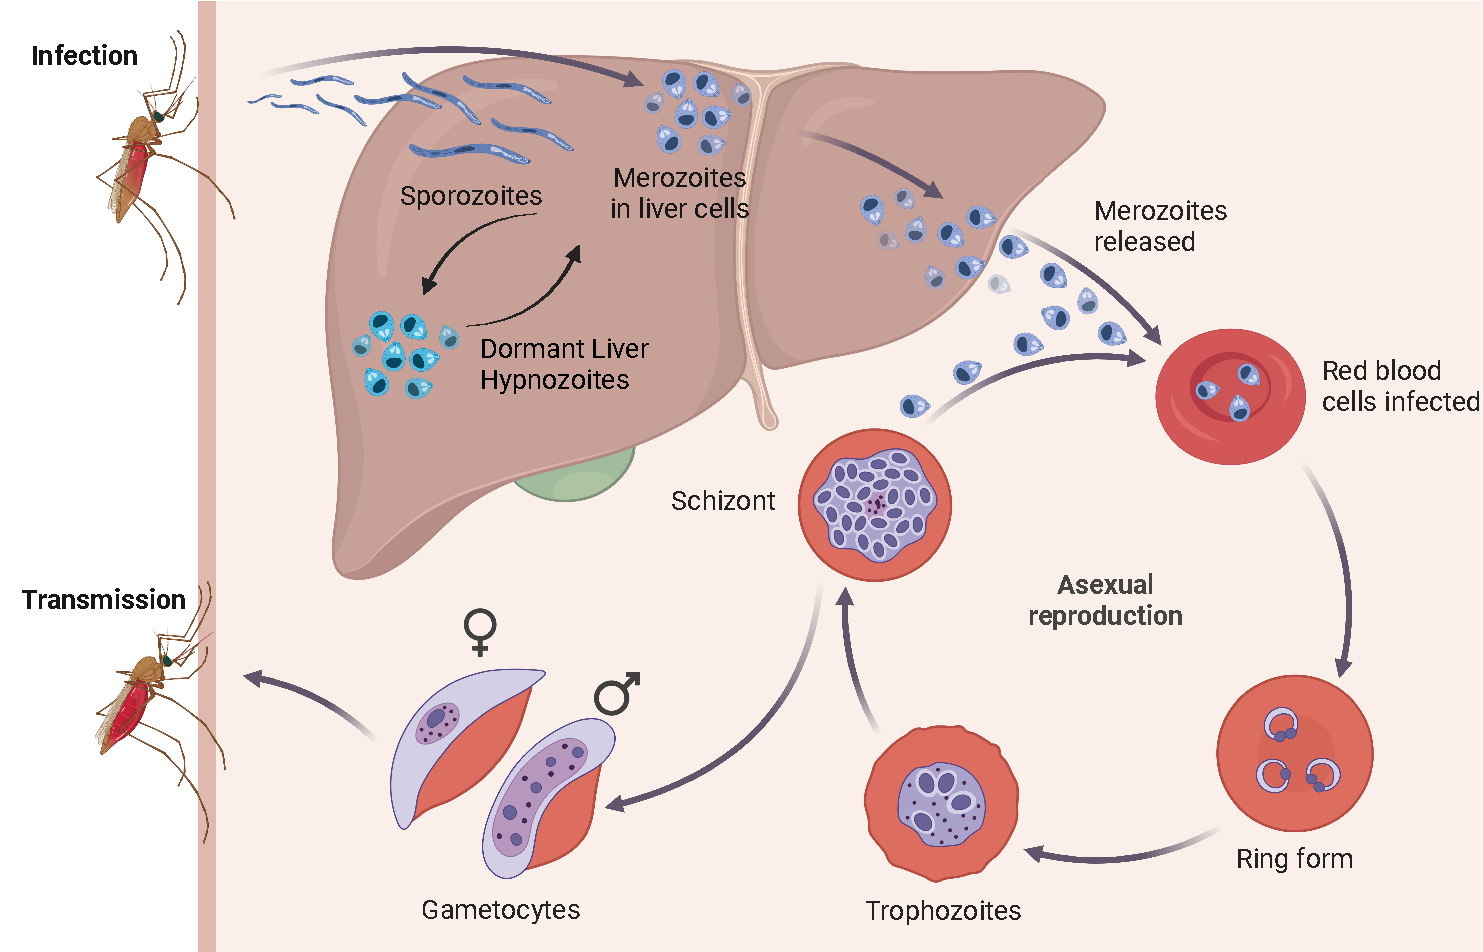
\includegraphics[width = \textwidth]{vivax_lifecycle_full.pdf}
    \caption{
        The \emph{P. vivax} (malaria) lifecycle. \emph{P. falciparum}
        does not have a dormant liver hypnozoite stage. Created with
        BioRender.com.
    }
    \label{fig:mal_lc}
\end{figure}

Malaria is a vector borne disease, needing both human (or other vertebrate) and
mosquito hosts to complete it's lifecycle (Figure \ref{fig:mal_lc}). Six
species of the unicellular parasite able to infect humans
\parencite{milner_malaria_2018}. Although \textit{Plasmodium falciparum} is
responsible for around 90\% of total human malaria deaths, outside of Africa
\textit{Plasmodium vivax} is the leading cause of malaria infection
\parencite{zekar_plasmodium_2023, adams_biology_2017}. Sporozoites (a stage of
the malaria parasite) enter the human blood stream via the skin after the
female mosquito has a blood meal. From the blood stream they proceed to enter
into the liver. Once a hepatocyte (liver cell) is invaded, the parasite will
undergo asexual reproduction into up to 40,000 merozoites per hepatocyte, which
are released into the blood stream . These merozoites then bind to, and invade
erythrocytes (red blood cells), once again reproducing 16-32 fold in a process
called schizogony. At this point, the erythrocyte membrane is ruptured,
allowing for \textit{Plasmodium} to invade new erythrocytes. Eventually, the
merozoites undergo sexual differentiation, resulting in the sequestration and
maturation of male and female gametocytes in the bone marrow, until they are
released into the blood stream to be consumed by a mosquito during a blood feed
where it matures into sporozoites ready to reinfect a new vertebrate host when
the mosquito next takes a blood feed \parencite{cowman_malaria_2016}.

\subsection*{Illness, Treatment, and Immunity}

The most common symptom of malaria infection in persons without natural or
acquired immunity is fever. After treatment, fever will usually subside over a
few days. In severe cases, malaria can lead to anemia, cerebral malaria (coma),
and respiratory distress \parencite{cowman_malaria_2016}.

In a population with stable malarial infection, immunity increases with age,
with the proportion of severe cases negligible after age 10, and asymptomatic
infection being the dominant infection type beyond age 15
\parencite{cowman_malaria_2016}.

\subsection*{Control and Eradication}

Widespread use of DDTs in the mid 20th century led to significant successes in
some countries towards the control and eradication of malaria. In the 1980s and
1990s, drug resistant malaria led to a doubling of malaria-attributable death.
Currently, the control techniques include insecticide treated bed nets, and a
mixture of antimalarial drugs \parencite{cowman_malaria_2016}.

\subsection*{\textit{Plasmodium vivax}}

Unlike \textit{P.\ falciparum}, \textit{P.\ vivax} has hypnozoites, which are a
dormant liver stage of the parasite. These can remain dormant for weeks and
even months, leading to recurrent infections and illness, possibily until the
conditions for transmission are more favourable. In subtropical/temperate
areas, the incubation periods can be between 8-12 months, compared to 3-4 weeks
in tropical regions. \cite{price_plasmodium_2020}. \textit{P.\ vivax} also has
lower levels of the blood stage parasite during infection, which means
diagnosis is more difficult, and it has an increased proportion of asymptomatic
cases \parencite{adams_biology_2017}.

It is likely that death and severe disease attributable to \textit{P.\ vivax}
has been traditionally underestimated. In view of recent evidence, the old
notion that \textit{P.\ vivax} is benign has become untenable
\parencite{cowman_malaria_2016}.

\subsection*{Motivating Malaria Models}

Levels of asymptomatic cases and latent parasite (in the case of
\textit{P.\ vivax}) are impossible or difficult to experimentally determine
without mass testing. By creating a model of the disease, and calibrating the
model so that it simulates symptomatic case levels reported by health
authorities, it is possible to estimate these previously `hidden' levels.
Furthermore, modelling malaria allows for modelling the effect of public health
interventions such as mass treatment or testing, in order to determine an
estimate of how effective the intervention may be, before large amounts of
money are spent on trials.

\section{Malaria Models}

\subsection*{Ross-Macdonald}

\begin{figure}[htbp]
    \centering
    \begin{tikzpicture}[thick]
        \node[draw, minimum size=1.5cm] (SH) {$S_\mathrm{H}$};
        \node[draw, right=of SH, minimum size=1.5cm] (IH) {$I_\mathrm{H}$};
        \node[draw, below=of SH, minimum size=1.5cm] (SM) {$S_\mathrm{M}$};
        \node[draw, below=of IH, minimum size=1.5cm] (IM) {$I_\mathrm{M}$};
        \draw[->] (SH) edge node [midway, label=above:{$\lambda_\mathrm{H}$}]
        (lambdaH) {} (IH);
        \draw[->] (SM) edge node [midway, label=below:{$\lambda_\mathrm{M}$}]
        (lambdaM) {} (IM);
        \draw[->, dashed, ruby] (IH) to (lambdaM);
        \draw[->, dashed, ruby] (IM) to (lambdaH);
        \draw[->] (IH) edge[in = 90, out = 90] node
        [midway, label=above:{$\gamma_\mathrm{H}$}] (omegaH) {} (SH);
        \node[below=of SM] (b_SM) {};
        \node[left=of SM] (l_SM) {};
        \node[below=of IM] (b_IM) {};
        \draw[->] (SM) edge node [midway, label=right:{$\mu_M$}] (SmuM) {} (b_SM);
        \draw[->] (l_SM) edge node [pos = 0.1, label=above:{$N_M\mu_M$}] (NmuM) {} (SM);
        \draw[->] (IM) edge node [midway, label=right:{$\mu_M$}] (ImuM) {} (b_IM);
    \end{tikzpicture}
    \caption{
        A simple Ross-Macdonald malaria model schematic, as described by
        \cite{aron_population_1982}. $S_\mathrm{H}$ and $I_\mathrm{H}$ are the
        number of susceptible and infected humans respectively, and
        $S_\mathrm{M}$ and $I_\mathrm{M}$ are the number of susceptible and
        infected mosquitos. The rate of human infection ($\lambda_\mathrm{H}$)
        is dependant on $I_\mathrm{M}$, and the rate of human infection
        ($\lambda_\mathrm{M}$) is dependant on $I_\mathrm{H}$.
    }
    \label{fig:ross_mac}
\end{figure}

Modelling malaria presents an additional challenge, as the disease is
transmitted from mosquito to human and human to mosquito, rather than having
direct human to human transmission. The most simple Ross-Macdonald model is
depicted in figure \ref{fig:ross_mac}. The ODEs for this model are
\begin{align*}
    \frac{\diff S_\mathrm{H}}{\diff t}
    = & \, \gamma_\mathrm{H}I_\mathrm{H}
    - bT_{\mathrm{HM}}I_\mathrm{M}\frac{S_\mathrm{H}}{N_\mathrm{H}}      \\
    \frac{\diff I_\mathrm{H}}{\diff t}
    = & \, bT_{\mathrm{HM}}I_\mathrm{M}\frac{S_\mathrm{H}}{N_\mathrm{H}}
    - \gamma I_\mathrm{H}                                                \\
    \frac{\diff S_\mathrm{M}}{\diff t}
    = & \, N_\mathrm{M}\mu_M + \gamma_\mathrm{M}I_\mathrm{M}
    - bT_{\mathrm{MH}}S_\mathrm{M}\frac{I_\mathrm{H}}{N_\mathrm{H}}
    - S_\mathrm{M}\mu_M                                                  \\
    \frac{\diff I_\mathrm{M}}{\diff t}
    = & \, bT_{\mathrm{MH}}S_\mathrm{M}\frac{I_\mathrm{H}}{N_\mathrm{H}}
    - \gamma_\mathrm{M}I_\mathrm{M}
\end{align*}
where $b$ is the biting rate per mosquito, and $T_{\mathrm{HM}}$ is the
probability of tranmission to a human given a bite by an infectious mosquito,
with $T_{\mathrm{MH}}$ being vice-versa. Note that it is
$\frac{I_\mathrm{H}}{N_\mathrm{H}}$ in the mosquito dynamics. Biologically this
is assuming the number of blood meals a mosquito takes per day is invariant to
the size of the human population. Mosquitos don't `recover' from malaria due to
their short lifespans, but the births and deaths are mathematically equivalent
to assuming that the rate of `recovery' amongst mosquitos is
$\mu_\mathrm{M}I_\mathrm{M}$ per unit time, with no population dynamics.

A Ross-Macdonald style model simplifies the lifecycle of malaria to the
following four steps \parencite{smith_ross_2012}: \begin{enumerate}
    \item Malaria is transmitted to human (or vertebrate) via a blood feed.
    \item Malaria proliferates in the human host until it circulates in the
          peripheral blood
    \item A mosquito then takes a blood feed, ingesting the pathogen
    \item Malaria develops within the mosquito host, progressing to its
          salivary glands, able to infect a human.
\end{enumerate}

\subsection*{Models of \textit{P.\ Vivax} Malaria}

\subsubsection*{White Model}

\begin{figure}[htbp]
    \centering
    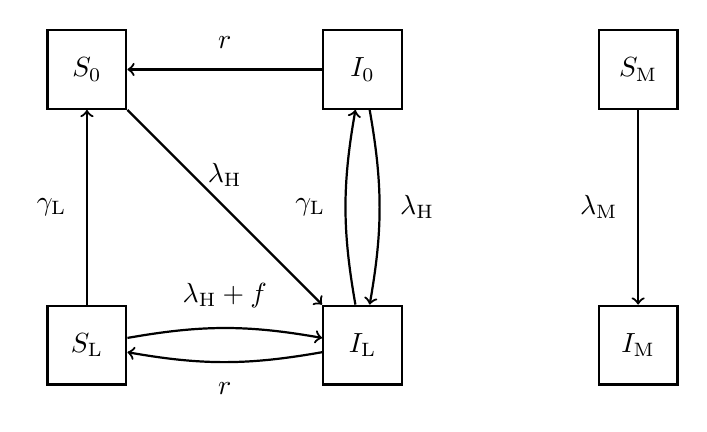
\begin{tikzpicture}[thick]
        \node[draw, minimum size=1cm] (S0) {$S_0$};
        \node[draw, right of=S0, minimum size=1cm, node distance=3.5cm] (I0)
        {$I_0$};
        \node[draw, below of=S0, minimum size=1cm, node distance=3.5cm] (SL)
        {$S_\mathrm{L}$};
        \node[draw, below of=I0, minimum size=1cm, node distance=3.5cm] (IL)
        {$I_\mathrm{L}$};
        \node[draw, right of=I0, minimum size=1cm, node distance=3.5cm] (SM)
        {$S_\mathrm{M}$};
        \node[draw, right of=IL, minimum size=1cm, node distance=3.5cm] (IM)
        {$I_\mathrm{M}$};
        \draw[->] (S0) edge node [midway, label=above:{$\lambda_\mathrm{H}$}]
        (lambdaH1) {} (IL);
        \draw[->] (SL) edge node [midway, label=left:{$\gamma_\mathrm{L}$}]
        (gammaL1) {} (S0);
        \draw[->] (SL) edge[in = 170, out = 10] node
        [midway, label=above:{$\lambda_\mathrm{H} + f$}] (lambdaf) {} (IL);
        \draw[->] (IL) edge[in = -10, out = 190] node
        [midway, label=below:{$r$}] (r) {} (SL);
        \draw[->] (IL) edge[in = 260, out = 100] node
        [midway, label=left:{$\gamma_\mathrm{L}$}] (gammaL2) {} (I0);
        \draw[->] (I0) edge[in = 80, out = 280] node
        [midway, label=right:{$\lambda_\mathrm{H}$}] (lambdaH2) {} (IL);
        \draw[->] (I0) edge node [midway, label=above:{$r$}] (r2) {} (S0);
        \draw[->] (SM) edge node [midway, label=left:{$\lambda_\mathrm{M}$}]
        (lambdaM) {} (IM);
    \end{tikzpicture}
    \caption{
        Diagram for \textit{P.\ vivax} model in a tropical setting described by
        \cite{white_variation_2016}. $S$ and $I$ are the number of susceptible
        and infected humans and mosquitos (denoted by subscript M).
        $\lambda_\mathrm{H} = mabI_\mathrm{M}$ and
        $\lambda_\mathrm{M} = ac(I_0 + I_\mathrm{L})$
    }
    \label{fig:white_2}
\end{figure}

The White model - described in \cite{white_variation_2016} (tropical model) and
depicted in Figure \ref{fig:white_2} - is characterised by the following
ordinary differential equations:

\begin{align*}
    \frac{\diff S_0}{\diff t}
    = & -\lambda_\mathrm{H} S_0 + rI_0 + \gamma_\mathrm{L}S_\mathrm{L} \\
    \frac{\diff I_0}{\diff t}
    = & -\lambda_\mathrm{H} I_0 - rI_0 + \gamma_\mathrm{L}I_\mathrm{L} \\
    \frac{\diff S_\mathrm{L}}{\diff t}
    = & -\lambda_\mathrm{H} S_\mathrm{L} + rI_\mathrm{L}
    - fS_\mathrm{L} -\gamma_\mathrm{L}S_\mathrm{L}                     \\
    \frac{\diff I_\mathrm{L}}{\diff t}
    = & \lambda_\mathrm{H} (S_0 + I_0 + S_\mathrm{L}) - rI_\mathrm{L}
    + fS_\mathrm{L} -\gamma_\mathrm{L}I_\mathrm{L}                     \\
    \frac{\diff S_\mathrm{M}}{\diff t}
    = & g - \lambda_\mathrm{M}(pS_\mathrm{M}
    - (1 - p)I_\mathrm{M}) - gS_\mathrm{M}                             \\
    \frac{\diff I_\mathrm{M}}{\diff t}
    = & \lambda_\mathrm{M}(pS_\mathrm{M} - (1 - p)I_\mathrm{M})
    - gI_\mathrm{M}
    \tag{$I_0 + I_\mathrm{L}=$ total number of bloodstage infections}.
\end{align*}

It modifies the Ross-Macdonald models, to capture the differences in disease
progression between \textit{P.\ vivax} and \textit{P.\ falciparum}.
In particular, the White model includes the dormant liver stage that is
unique to \textit{P.\ vivax}.

The model is comprised of six compartments: \begin{enumerate}
    \item \textbf{
              $S_0$ (Susceptible Individuals - No Latent Hypnozoite Liver
              Stage Infection)
          }: People in this compartment have no form of malarial infection.
          These people are susceptible to new malarial infections,
          and are infected into compartment $I_\mathrm{L}$ (with both blood
          and liver stage parasites) with rate $\lambda_\mathrm{H}$.
    \item \textbf{
              $I_\mathrm{L}$ (Infected Individuals - Both Blood Stage and Latent
              Hypnozoite Liver Stage Infection)
          }:  Individuals in this compartment have both an active blood-stage
          infection, and latent hypnozoite infection in the liver. They can
          progress to either $I_0$ through the clearance of liver stage
          infection with rate $\gamma_\mathrm{L},$ or to $S_\mathrm{L}$ through
          clearance of blood stage infection with rate $r$.
    \item \textbf{
              $I_0$ (Infected Individuals - Blood-Stage Infection Only)
          }: Those in this compartment have a blood-stage infection with no
          latent hypnozoite infection in the liver. They are be reinfected into
          $I_\mathrm{L}$ with rate $\lambda_\mathrm{H}$, relapse with rate $f$.
          Blood-stage infection is cleared (moving into compartment $S_0$) with
          rate $r$.
    \item \textbf{
              $S_\mathrm{L}$ (Susceptible Individuals -
              Blood-Stage Infection Only)
          }: Those in this compartment have latent hypnozoite infection in
          the liver without blood-stage infection. They get novel infection
          through a mosquito bite into $I_\mathrm{L}$ with rate
          $\lambda_\mathrm{H}$, or hypnozoite activation with rate $f$.
          This means that those in $S_\mathrm{L}$ move to compartment
          $I_\mathrm{L}$ with total rate $\lambda_\mathrm{H} + f.$
          Alternatively the hypnozoites are cleared from the liver
          (moving to compartment $S_0$) with rate $\gamma_\mathrm{L}.$
    \item \textbf{
              $S_\mathrm{M}$ (Susceptible Mosquitoes)
          }:
          Suspectable mosquitoes become infectious at rate
          $\lambda_\mathrm{M}p.$ They die at rate
          $g + \lambda_\mathrm{M}(1 - p).$ Since there is a constant mosquito
          population assumption, mosquitoes are born into this state at rate
          $g + \lambda_\mathrm{M}.$
    \item \textbf{$I_\mathrm{M}$ (Infectious Mosquitoes)}:
          Infectious mosquitos die at rate $g + \lambda_\mathrm{M}(1 - p).$
\end{enumerate}

$\lambda_\mathrm{H} := mabI_\mathrm{M}$ where $m$ is the number of mosquitos
per human (held constant since there is no birth or death in the human
dynamics), $a$ is the mosquito biting rate, and $b$ is the probability that a
human bitten by an infectious mosquito develops an infection.

$\lambda_\mathrm{M} := ac(I_0 + I_\mathrm{L})$ where $a$ is defined above,
and $c$ is the probability that a mosquito bite on an infectious mosquito
causes the mosquito to become infectious. $g$ can be interpreted as the natural
birth/death rate for mosquitos. $p$ is then the proportion of mosquitos that
survive long enough after the initial infection that the parasite matures
enough in the mosquito before becoming infectious to new susceptible humans.
Under the assumption that time until parasite transmissability after
infection in a mosquito is a constant $n$ days, and that mosquitoes naturally
die at rate $g$, $p=e^{-gn}.$ To see this let $V\sim\mathrm{Exp}(g),$
represent the lifespan of the mosquito.
$\Pr(V > n)= 1 - F_V(n) = 1 - (1 - e^{-gn}) = e^{-gn}.$

$\lambda_\mathrm{M}(1 - p)$ can be interpreted as an additional rate of death,
where of the mosquitos that would develop malaria after a bite, a proportion
$1 - p$ die instantly. This applies to both the susceptible and infectious
mosquitoes. Presumably this approximates a model where mosquitoes are moved
to an `exposed' compartment for $n$ time, after initial infection,
however no justification is given in \parencite{white_variation_2016} for
this additional parameter $n$. A more straightforward $SI$ model could be
constructed that absorbs $c$ and $n$ into the single parameter $c^*$, such
that it becomes the proportion of mosquito bites on blood stage infectious
humans that result in mosquito infection where the mosquito does not die
before becoming infectious. With steady mosquito population, the mosquito
dynamics would now be characterised by
$$
    \frac{\diff I_\mathrm{M}}{\diff t}
    = \lambda_\mathrm{M}^*S_\mathrm{M} - gI_\mathrm{M}
    \quad\text{where } \lambda_\mathrm{M}^*:= ac^*(I_0 + I_\mathrm{L}).
$$

By modelling both liver and bloodstage infection, blood stage infections
from relapses can be captured in the dynamics, meaning it is possible to
analyse case number data that may be confounded by relapses as well as
novel infections.

% Combining this model with pre-established within host dynamics, the 
% model allows for analysis of how the hypnozoite activation rate 
% (closely related to relapse frequency) can effect the total number of 
% relapsing hypnozoites, the time with liver stage infection, and the basic 
% reproduction number $R_0$ (important particularly in considering interventions
%  and potential evolutionary strain selection).

This model does not account for continual depletion of liver stage parasites
which would vary the rate of relapse over time (through clearance or relapse).
It also does not directly model any interventions or case importations. The
lack of population dynamics means the model may only be useful on a small time
scale. Finally, it doesn't account for any importation of disease from an
outside area, so if $S_0 = 1,$ \textit{P.\ vivax} is presumed permanently
eradicated.

\subsubsection*{Champagne Model}\label{sec:champ_mod}

\begin{figure}[htbp]
    \centering
    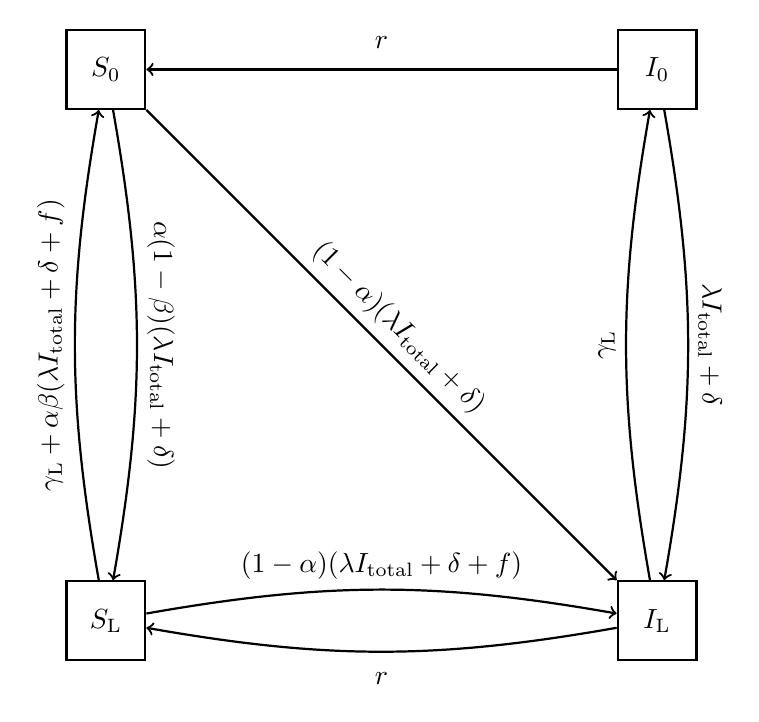
\begin{tikzpicture}[thick]
        \node[draw, minimum size=1cm] (S0) {$S_0$};
        \node[draw, right of=S0, minimum size=1cm, node distance=7cm] (I0) {$I_0$};
        \node[draw, below of=S0, minimum size=1cm, node distance=7cm] (SL) {$S_\mathrm{L}$};
        \node[draw, below of=I0, minimum size=1cm, node distance=7cm] (IL) {$I_\mathrm{L}$};
        \draw[->] (S0) edge[sloped] node[above] {$(1 - \alpha)(\lambda I_\mathrm{total} + \delta)$} (IL);
        \draw[->] (S0) edge[in = 80, out = 280, sloped] node[above] {$\alpha( 1 -\beta)(\lambda I_\mathrm{total} + \delta)$} (SL);
        \draw[->] (SL) edge[in = 260, out = 100, sloped] node [above] {$\gamma_\mathrm{L} + \alpha\beta(\lambda I_\mathrm{total} + \delta + f)$} (S0);
        \draw[->] (SL) edge[in = 170, out = 10, sloped] node [above] {$(1 -\alpha)(\lambda I_\mathrm{total} + \delta + f)$} (IL);
        \draw[->] (IL) edge[in = -10, out = 190] node [midway, label=below:{$r$}] (r) {} (SL);
        \draw[->] (IL) edge[in = 260, out = 100, sloped] node [above] {$\gamma_\mathrm{L}$} (I0);
        \draw[->] (I0) edge[in = 80, out = 280, sloped] node [above] {$\lambda I_\mathrm{total} + \delta$} (IL);
        \draw[->] (I0) edge node [midway, label=above:{$r$}] (r2) {} (S0);
    \end{tikzpicture}
    \caption{Diagram for \textit{P.\ vivax} model described by \cite{champagne_using_2022}. $I_\mathrm{total} = I_0 + I _\mathrm{L}.$ Since the mosquito dynamics have been removed, $\lambda$ now not has no dependencies on the number of infectious mosquitos.}\label{fig:champ_diag}
\end{figure}

The Champagne model - described in \parencite{champagne_using_2022} and diagrammatically depicted in figure \ref{fig:champ_diag} - both simplifies and extends the White model. The model assumes human to human transmission, removing mosquito dynamics, and extends it by adding in a rate of imported cases and treatment of malarial infection. It is characterised by the system of ordinary differential equations
\begin{align*}
    \frac{\diff I_\mathrm{L}}{\diff t} = & (1 - \alpha)(\lambda I_\mathrm{total} + \delta)(S_0 + S_\mathrm{L}) + (\lambda I_\mathrm{total} + \delta)I_0 + (1 - \alpha)fS_\mathrm{L} - \gamma_\mathrm{L}I_\mathrm{L} - rI_\mathrm{L}  \\
    \frac{\diff I_0}{\diff t} =          & -(\lambda I_\mathrm{total} + \delta)I_0 + \gamma_\mathrm{L}I_\mathrm{L} - rI_0                                                                                                            \\
    \frac{\diff S_\mathrm{L}}{\diff t} = & -(1 - \alpha(1 - \beta))(\lambda I_\mathrm{total} + \delta + f)S_\mathrm{L} + \alpha(1-\beta)(\lambda I_\mathrm{total} + \delta)S_0 - \gamma_\mathrm{L}S_\mathrm{L} + rI_\mathrm{L}       \\
    \frac{\diff S_0}{\diff t} =          & -(1 - \alpha\beta)(\lambda I_\mathrm{total} + \delta)S_0 + (\lambda I_\mathrm{total} + \delta)\alpha\beta S_\mathrm{L} + \alpha\beta fS_\mathrm{L} + \gamma_\mathrm{L}S_\mathrm{L} + rI_0
\end{align*} where $I_\mathrm{total} := I_0 + I_\mathrm{L}.$

The compartments have the same interpretation as in the White model, however the rates between compartments are significantly modified.

The new parameters are $\lambda:$ the rate of infection,
$\delta:$ importation rate,
$\alpha:$ proportion of those infected who clear blood stage
infections through immediate treatment, and
$\beta:$ proportion of those cleared of blood stage infection who
are also cleared of liver stage parasites (radical cure)
In other words, the proportion of infected individuals $\alpha\beta$ are
completely cured from liver and blood stage parasites. The model assumes
treatment clears infection instantaneously. Individuals in $S_\mathrm{L}$ who
relapse or get a new infection are assumed to be cured with the same
proportions as new infections from $S_0,$ but individuals in $I_0$ who are
superinfected are assumed not to seek treatment.

In contrast to the White model, the Champagne model allows analysis of potential treatment interventions, or how much of an impact limiting the importation rate might have on case numbers (through border control/testing). Although the lack of mosquito dynamics simplifies the model and it's running, it is unrealistic. The model still has some of the same problems as the White model, such as not incorporating hypnozoite depletion rates and a lack of population dynamics, meaning all analytic results are done assuming the system is at equilibrium.